\chapter{Wind Tunnel Testing}
\label{ch:windTunnel}
\label{sec:wtDAQ}

This chapter describes the wind-tunnel testing of MARGE and the post-processing of the wind tunnel test data.

MARGE was tested at the University of Washington's 3x3 low-speed wind tunnel at six flight conditions, $q_D=\{60,100,163,207,281,343\}$ Pa. At each flight condition, the response to each of the four inputs was tested three times. For the gust vanes, a discrete 4-degree doublet gust was generated with a frequency of 1.45 Hz (approximately equivalent to the first wing bending natural frequency). For the ailerons, a 5-degree frequency sweep from 1 Hz to 2 Hz was performed. For the elevator, a 2-degree frequency sweep from 1 Hz to 2 Hz was performed. The sweep's frequency band was chosen to encompass the first wing bending mode while staying within the bandwidth of the actuators.

The exception to the above is at $q_D=343$ Pa. At this dynamic pressure, the aileron sweeps were reduced in magnitude to 3.5 degrees and the elevator sweep was reduced in magnitude to 1 degree. This was done in order to reduce the risk of damage to the model due to violent responses at high speeds.

All of these tests were controlled and recorded using Simulink Real-Time. The testing yielded time-series data of input commands and sensor readings for each test. An example of a single run of data is shown in Fig. \ref{fig:sampleWT}
\begin{figure}[H]
	\centering
	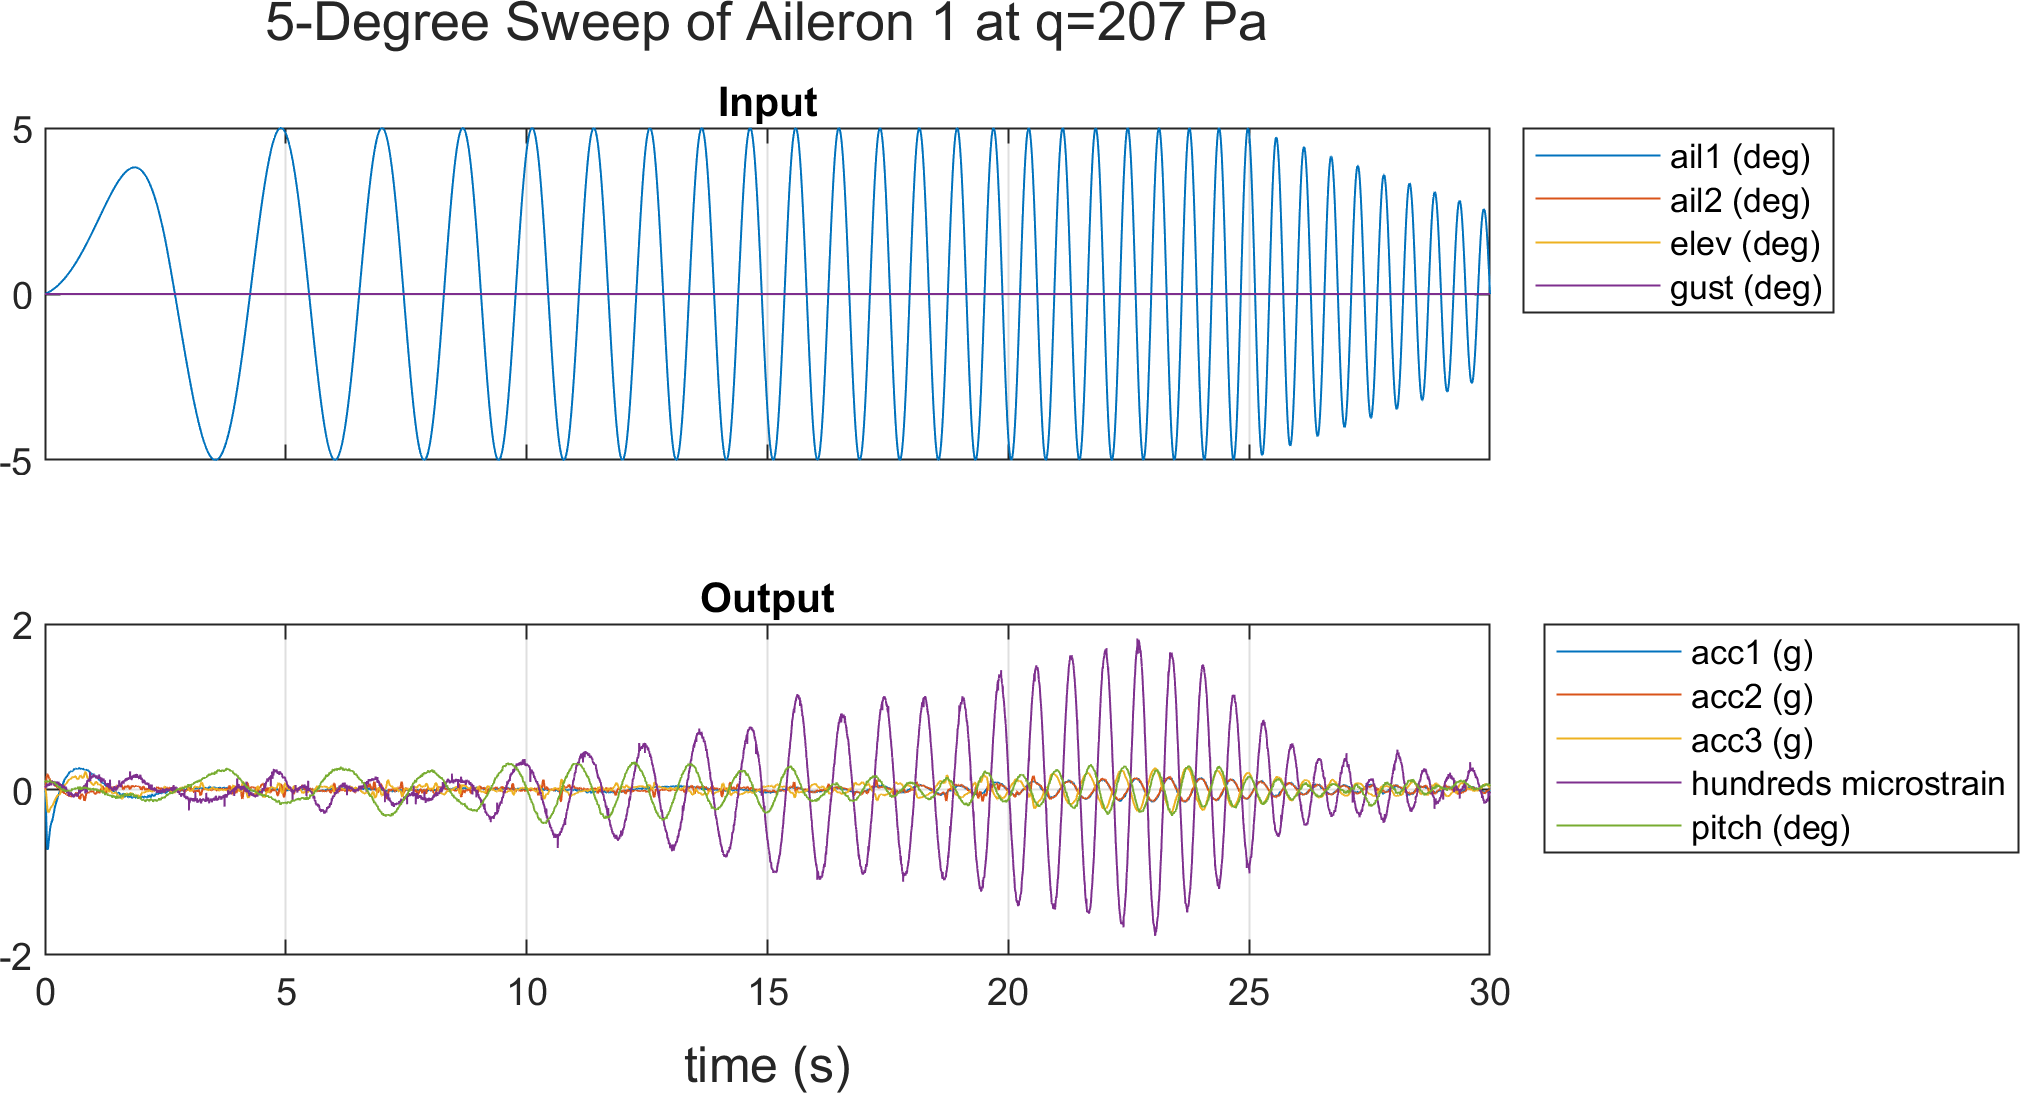
\includegraphics[width=6in]{figs/sampleWT.png}
	\caption{Sample wind tunnel time-series data from a single run}
	\label{fig:sampleWT}
\end{figure}

%%%%%%%%%%%%%%%%%%%%%%%%%%%%%%%%%%%%%%%%%%%%%%%%%%%%%%%%%%%%%%%%%%%%
\section{Data Postprocessing} %%%%%%%%%%%%%%%%%%%%%%%%%%%%%%%%%%%%%%
%%%%%%%%%%%%%%%%%%%%%%%%%%%%%%%%%%%%%%%%%%%%%%%%%%%%%%%%%%%%%%%%%%%%

The time-domain data was post-processed in a similar way as was done for the GVT data in Section \ref{sec:generateFRF}. Each run's data was truncated to start when the input began and end five seconds after the input ended. The data was re-centered to have zero mean and then the three runs of each test were concatenated.

This single concatenated time-domain signal was then buffered into overlapping Hann windows and transformed using the CZT. The FRFs were then computing using Equation \ref{eq:frf}. The FRFs were computed from 0.4 Hz to 2.0 Hz.

\subsection{Accelerometer Data Postprocessing} %%%%%%%%%%%%%%%%%
\label{sec:accDataPost}

The output of the accelerometers contained significant noise and potentially contained electrical interference from other components in MARGE. Thus, the uncertainty in FRFs between inputs and the accelerometers was high. This was compensated for by specifically filtering the time-series signal from accelerometers before other postprocessing and limiting the bandwidth of the FRFs produced to within a range in which the accelerometers tend to behave more consistently.
%The shortcomings in the hardware of MARGE, including the accelerometers, will be discussed further in Section \ref{sec:shortcomings}.

Before going through the postprocessing steps outlined above, the time-series signal from the accelerometers was filtered using a Butterworth bandpass filter which limited frequencies in the signal to between 0.8 Hz and 25 Hz. This was done to reduce the effect of both high-frequency noise and low-frequency drift in the acclerometer signals. This same bandpass filter was applied to the input signal when generating FRFs between an input and the accelerometers so that the filter would not skew the FRF.

Unlike for other input-output combinations, all FRFs of an input to an accelerometer were only computed between 1 Hz and 2 Hz in the frequency domain. This was because the $H_1$ and $H_2$ FRFs diverged significantly outside of these bounds, indicating high uncertainty in the FRFs due to issues in the data (such as noise).